\documentclass[12pt, a4paper, times, capchap, capsec, floatnumber=continuous, header=yes]{abnt}
\usepackage[utf8]{inputenc} % acentos em portugues
\usepackage{graphicx} % importar imagens
\usepackage{sty/abnt-UFSC}
\usepackage{longtable,color}
\usepackage{amsmath}
\newcommand{\norm}[1]{\left\lVert#1\right\rVert}
\usepackage{amstext}
\usepackage{amsfonts}
\usepackage{amssymb}
\usepackage{array}
\usepackage{hyphenat}
\usepackage{url}
\usepackage{caption}
\usepackage{float}
\usepackage{listings}
\usepackage{textcomp}

\lstset{language=C,
numbers=left,
stepnumber=1,
firstnumber=1,
numberstyle=\tiny,
extendedchars=true,
breaklines=true,
frame=tb,
basicstyle=\footnotesize,
stringstyle=\ttfamily,
showstringspaces=false
}
\renewcommand{\lstlistingname}{C\'{o}digo Fonte}
\renewcommand{\lstlistlistingname}{Lista de C\'{o}digos Fonte}

\def\Versao$#1 #2${#2}
\def\Data$#1 #2 #3${#2}

\autor{Vitor Arins Pinto}
\titulo{Redes Neurais Convolucionais de Profundidade para Reconhecimento de Textos em Imagens de CAPTCHA.}
\orientador[]{Orientadora: Luciana de Oliveira Rech }
\comentario{Trabalho de Conclusão de Curso submetido ao Programa de
  graduação da Universidade Federal de Santa Catarina para a obtenção
  do Grau de Bacharel em Sistemas de Informação.}
\instituicao{Universidade Federal de Santa Catarina \par
    Centro Tecnológico \par
    Departamento de Informática e Estatística}
\local{Florian\'{o}polis}
\data{\today}


\begin{document}

\capa
\folhaderosto

\chapter*{Agradecimentos}

Primeiramente gostaria de agradecer à minha amada namorada e melhor
amiga Letícia, que além de me mostrar o real significado do amor e
me apresentar a felicidade de uma maneira que eu não conhecia,
cooperou no desenvolvimento do trabalho desde o seu início, suportando
amorosamente a minha ausência, se sobrecarregando com trabalho
(inclusive o de revisar esse texto) permitindo que eu me dedicasse
integralmente ao desenvolvimento do mesmo.

Aos meus pais agradeço por todo o esforço e sacrifício que fizeram
para que eu pudesse chegar aqui, sem eles eu certamente não teria
oportunidade de realizar este trabalho nem de viver todas as
experiências maravilhosas que tive até hoje.

Ao meu irmão Marcel por tudo que me ensinou e todos os conselhos que
me deu até hoje.

Agradeço à Marilene Bittencourt que sempre me incentivou a ser melhor
e há muito tempo dá ensinamentos que me levam para um caminho de
sucesso.

Ao meu mentor Eduardo Bellani por me guiar nos primeiros momentos
profissionais de minha carreira.

Agradeço a Neoway e todos os seus funcionários pelas oportunidades que
me foram dadas e por fornecer dados indispensáveis no desenvolvimento
deste trabalho.

Por fim agradeço a todos os professores da UFSC que tive contato, em
especial a minha orientadora Prof.ª Luciana de Oliveira Rech, Dr.ª e aos
membros da banca Prof. Mário Antônio Ribeiro Dantas, Dr. e Prof.ª 
Jerusa Marchi, Dr.ª.
\begin{resumo}
        
Atualmente, muitas aplicações na Internet seguem a política de manter
alguns dados acessíveis ao público. Para isso é necessário desenvolver
um portal que seja robusto o suficiente para garantir que todas as
pessoas possam acessá-lo. Porém, as requisições feitas para recuperar
dados públicos nem sempre vêm de um ser humano. Empresas
especializadas em Big data possuem um grande interesse em fontes de
dados públicos para poder fazer análises e previsões a partir de dados
atuais. Com esse interesse, \textit{Web Crawlers} são
implementados. Eles são responsáveis por consultar fontes de dados
milhares de vezes ao dia, fazendo diversas requisições a um
\textit{website}. Tal \textit{website} pode não estar preparado para
um volume de consultas tão grande em um período tão curto de
tempo. Com o intuito de impedir que sejam feitas consultas por
programas de computador, as instituições que mantêm dados públicos
investem em ferramentas chamadas CAPTCHA (teste de Turing público
completamente automatizado, para diferenciação entre computadores e
humanos). Essas ferramentas geralmente se tratam de imagens contendo
um texto qualquer e o usuário deve digitar o que vê na imagem. O
objetivo do trabalho proposto é realizar o reconhecimento de texto em
imagens de CAPTCHA através da aplicação de redes neurais
convolucionais.

\end{resumo}

\begin{abstract}

Currently many applications on the Internet follow the policy of keeping
some data accessible to the public. In order to do this, it's
necessary to develop a portal that is robust enough to ensure that all
people can access this data. But the requests made to recover
public data may not always come from a human. Companies
specializing in Big data have a great interest in data from public
sources in order to make analysis and forecasts from current 
data. With this interest, Web Crawlers are implemented. They are
responsible for querying data sources thousands of times a day,
making several requests to a website. This website may not be
prepared for such a great volume of inquiries in a short period of
time. In order to prevent queries to be made by
computer programs, institutions that keep public data
invest in tools called CAPTCHA (Completely Automated Public
 Turing test to tell Computers and Humans Apart). These tools usually deal
with images containing text and the user must enter what he or she
sees in the image. The objective of the proposed work is to perform the
text recognition in CAPTCHA images through the application of
convolutional neural networks.

\end{abstract}


\listoffigures
\listoftables
% Para seguir um padrão, a lista de siglas fica em um arquivo
% separado e todas a suas configurações específicas são colocados
% neste arquivo.

\chapter*{Lista de abreviaturas e siglas}

\noindent
\verb"CAPTCHA" \dotfill \textit{Completely Automated Public Turing
  test to tell Computers and Humans Apart}\\
\verb"HDF" \dotfill \textit{Hierarchical Data Format}\\
\verb"GPU" \dotfill \textit{Graphics Processing Unit}\\
\verb"AWS" \dotfill \textit{Amazon Web Services}\\
\verb"IA" \dotfill \textit{Inteligência Artificial}\\
\verb"DCNN" \dotfill \textit{Deep Convolutional Neural Networks}\\
\verb"ReLU" \dotfill \textit{Rectified Linear Unit}\\

\sumario

\setcounter{page}{1}

\chapter{Introdução}

Redes neurais artificiais clássicas existem desde os anos 60, como fórmulas  
matemáticas e algorítimos. Atualmente os programas de aprendizado de máquina  
contam com diferentes tipos de redes neurais. Um tipo de rede neural muito  
utilizado para processamento de imagens é a rede neural convolucional de  
profundidade. O trabalho em questão tratará da utilização e
configuração de uma rede neural convolucional de profundidade para
reconhecimento de textos em imagens específicas de CAPTCHAs.

\section{Problema}

Com o aumento constante na quantidade de informações geradas e 
computadas atualmente, percebe-se o surgimento de uma necessidade de tornar
alguns tipos de dados acessíveis a um público maior. A fim de gerar
conhecimento, muitas instituições desenvolvem portais de acesso para
consulta de dados relevantes a cada pessoa. Esses portais, em forma de
aplicações na Internet, precisam estar preparados para receber
diversas requisições e em diferentes volumes ao longo do tempo.

Devido a popularização de ferramentas e aplicações especializadas em Big
data, empresas de tecnologia demonstram interesse em recuperar grandes
volumes de dados de diferentes fontes públicas. Para a captura de tais
dados, Web crawlers são geralmente implementados para a realização de
várias consultas em aplicações que disponibilizam dados públicos.

Para tentar manter a integridade da aplicação, as organizações que possuem  
estas informações requisitadas investem em ferramentas chamadas CAPTCHA  
(teste de Turing público completamente automatizado para diferenciação entre  
computadores e humanos). Essas ferramentas frequentemente se tratam de  
imagens contendo um texto qualquer e o usuário precisa digitar o que vê na  
imagem. 

O trabalho de conclusão de curso proposto tem a intenção de retratar a  
ineficiência de algumas ferramentas de CAPTCHA, mostrando como redes neurais  
convolucionais podem ser aplicadas em imagens a fim de reconhecer o texto  
contido nestas imagens. 

\section{Objetivos}

\subsection{Objetivo geral}

Analisar o treinamento e aplicação de redes neurais convolucionais de
profundidade para o reconhecimento de texto em imagens de CAPTCHA.

\subsection{Objetivos específicos}

\begin{itemize}
        \item Estudar trabalhos correlatos e analisar o estado da arte;
	\item Entender como funciona cada aspecto na configuração de
          uma rede neural convolucional;
	\item Realizar o treinamento e aplicação de uma rede neural
          artificial para reconhecimento de CAPTCHAs.
\end{itemize}

\section{Escopo do trabalho}

O escopo deste trabalho inclui o estudo e análise de uma rede neural
convolucional de profundidade para reconhecimento de texto em imagens de 
um CAPTCHA específico.

Não está no escopo do trabalho:

\begin{itemize}
  \item Analisar outras formas de inteligência no reconhecimento de
    texto. 
  \item O estudo, análise ou implementação da aplicação de redes
    neurais convolucionais para outros tipos de problemas. 
  \item O estudo, análise ou implementação de softwares do tipo
    ``crawler'' ou qualquer programa automatizado para recuperar
    quaisquer informações de websites públicos.
  \item A análise e comparação de diferentes técnicas ou parâmetros
    para otimização de redes neurais.
\end{itemize}

\section{Metodologia}

Para realizar o proposto, foram feitas pesquisas em base de dados tais
como IEE Xplorer e ACM Portal. Adquirindo assim maior conhecimento
sobre o tema, estudando trabalhos relacionados. 

Com base no estudo do estado da arte, foram feitas pesquisas e
estudos para indicar caminhos possíveis para desenvolvimento da
proposta de trabalho.

\section{Estrutura do trabalho}

Para uma melhor compreensão e separação dos conteúdos, este trabalho
está organizado em 6 capítulos. Sendo este o capítulo 1 cobrindo a
introdução ao tema, citando os objetivos e explicando a proposta.

O capítulo 2 apresenta a fundamentação teórica, com as definições das
abordagens de desenvolvimento de aprendizado de máquina e redes
neurais. Os conceitos de tipos de redes neurais.

No capítulo 3 está a proposta de experimento a ser realizado. Assim
como uma breve ideia dos resultados esperados e a forma de avaliação
dos mesmos.

O capítulo 4 contém as informações do desenvolvimento do sistema de
reconhecimento de imagens de CAPTCHA. Também a apresentação dos dados
obtidos através das metodologias escolhidas na seção anterior.

No capítulo 5 são apresentados os resultados da aplicação do sistema
de reconhecimento de imagens de CAPTCHA.

Por fim, no capítulo 6 estão as conclusões obtidas através dos
resultados deste trabalho, as ameaças que podem comprometer o acesso à
dados públicos disponbilizados e as sugestões para trabalhos futuros
relacionados.
\chapter{Fundamentação Teórica}

\section{Aprendizado de máquina}

Aprendizado de máquina, ou \textit{Machine Learning}, é uma área da
computação que emergiu de estudos relacionados ao reconhecimento de
padrões e inteligência artificial. Nesta área é contemplado o estudo e
implementação de algoritmos que conseguem aprender e fazer previsões
baseadas em dados. Esses algoritmos funcionam através da construção de
um modelo preditivo que tem como entrada um conjunto de treinamento
com dados de observações quaisquer. Desse modo as previsões são feitas
orientadas aos dados e não a partir de instruções estáticas de um
programa.

\section{Redes Neurais}

Diante das ferramentas disponíveis que tratam de aprendizado de
máquina, uma delas é a rede neural artificial.

Redes neurais artificiais são conjuntos de modelos inspirados por
redes neurais biológicas, usados para aproximar funções que dependem
de um número muito grande de entradas. De acordo com Mackay\cite{Mackay},
Redes neurais geralmente são especificadas utilizando 3 coisas:

\begin{itemize}

\item {\bf Arquitetura:} Especifica quais variáveis estão envolvidas
  na rede e quais as relações topológicas. Por exemplo, as variáveis
  envolvidas em uma rede neural podem ser os pesos das conexões entre
  os neurônios.

\item {\bf Regra de atividade:} A maioria dos modelos de rede neural
  tem uma dinâmica de atividade com escala de tempo curta. São regras
  locais que definem como as ``atividades'' de neurônios mudam em
  resposta aos outros. Geralmente a regra de atividade depende dos
  parâmetros da rede.

\item {\bf Regra de aprendizado:} Especifica o modo com que os pesos
  da rede neural muda conforme o tempo. O aprendizado normalmente toma
  uma escala de tempo maior do que a escala referente a dinâmica de
  atividade. Normalmente a regra de aprendizado dependerá das
  ``atividades'' dos neurônios. Também pode depender dos valores
  que são objetivos definidos pelo usuário e valores iniciais dos
  pesos.

\end{itemize}

Tomando imagens como exemplo, uma rede neural para reconhecimento de
texto pode ter como entrada o conjunto de pixels\footnote{pixel é o
  menor ponto que forma uma imagem digital, sendo que o conjunto de
  milhares de pixels formam a imagem inteira. Cada Pixel é composto
  por um conjunto de 3 pontos: verde, vermelho e azul.} da
imagem. Depois de serem atribuídos os pesos para cada item da entrada,
os próximos neurônios serão ativados mediante a função de atividade
pré-definida. Os pesos são recalculados através da regra de
aprendizado e todo processo é repetido até uma condição determinada
pelo usuário.

\section{Regressão logística multinomial}

Regressão logística multinomial é um método de classificação que
consiste em um modelo que é usado para prever probabilidades de
variáveis associadas a uma determinada classe, baseado em um conjunto
de variáveis independentes. Para construir este modelo, esta seção
descreve as tarefas e cálculos principais.

\subsection{Classificação supervisionada}

Classificação é uma tarefa central para o aprendizado de máquina, e
consiste em receber uma entrada, como a imagem da letra ``A'' por
exemplo, e dar um rótulo que diz que essa imagem é da classe
``A''. Geralmente temos muitos exemplos da entidade que queremos
classificar. Esses exemplos já mapeados com seu respectivo rótulo, são
chamados de conjunto de treinamento. Após o treinamento o objetivo é
receber um exemplo completamente novo e descobrir em qual classe esse
exemplo se encaixa.

Dizemos que esse aprendizado é supervisionado pois cada exemplo
recebeu um rótulo durante o treinamento. Ao contrário deste, o
aprendizado não supervisionado não conhece os rótulos de cada exemplo,
mas tenta agrupar os exemplos que possuem semelhança baseado em
propriedades úteis encontradas ao longo do treinamento.

\subsection{Classificador Logístico}

Um classificador logístico, ou linear, recebe como entrada os pixels
de uma imagem por exemplo, e aplica uma função linear a eles para
gerar suas predições. Uma função linear é apenas uma grande
multiplicação de matriz. Recebe todas as entradas como um grande vetor
que será chamado de ``X'', e multiplica os valores desse vetor com uma
matriz para gerar as predições, cada predição é como uma pontuação,
que possui o valor que indica o quanto as entradas se encaixam em uma
classe de saída.

\begin{equation}
   WX + b = Y
\end{equation}

``X'' é como chamaremos nosso vetor das entradas, ``W'' serão pesos e
o termo tendencioso (\textit{bias}) será representado por ``b''. ``Y''
corresponde ao vetor de pontuação para cada classe. Os pesos da
matriz e o \textit{bias} é onde age o aprendizado de máquina, ou seja,
é necessário tentar encontrar valores para os pesos e para o
\textit{bias} que terão uma boa performance em fazer predições para as
entradas.

\subsection{Função Softmax}

Como cada imagem pode ter um e somente um rótulo possível, é necessário
transformar essas pontuações em probabilidades. Queremos que a
probabilidade de ser a classe correta seja muito perto de {\bf 1.0} e
a probabilidade para todas as outras classes fique perto de {\bf
  0.0}.
Para tornar essas pontuações em probabilidades utilizamos uma função
chamada {\bf \emph{Softmax}}. Denotada na equação por ``S''.

\begin{equation}
   S(y_i) = \displaystyle\frac{e^{y_i}}{\displaystyle\sum_{j} e^{y_j}}
\end{equation}

O mais importante dessa fórmula é que pode receber qualquer tipo de
pontuação gerado por predições e transformá-la em probabilidades
adequadas. Os valores dessas probabilidades serão altos quando a
pontuação da classe for alta e baixos quando a pontuação da classe for
baixa. A soma das probabilidades fica igual a 1.

Ao final do processo de aplicação da função linear e da função
Softmax temos um vetor de tamanho igual ao número de classes possíveis
e em cada posição do vetor temos a probabilidade para a classe
referente a essa específica posição do vetor.

\subsection{One-Hot Encoding}

Para facilitar o treinamento é preciso representar de forma matemática
os rótulos de cada exemplo que iremos alimentar a rede neural. Cada
rótulo será representado por um vetor de tamanho igual ao número de
classes possíveis, assim como o vetor de probabilidades. No caso dos
rótulos, será atribuído o valor de {\bf 1.0} para a posição referente
a classe correta daquele exemplo e {\bf 0.0} para todas as outras
posições. Essa tarefa é bem simples e geralmente chamada de
\textit{One-Hot Encoding}. Com isso é possível medir a eficiência do
treinamento apenas comparando 2 vetores.

\subsection{Cross Entropy}

O jeito mais comum em redes neurais de profundidade para medir a
distância entre o vetor de probabilidades e o vetor correspondente ao
rótulo se chama {\bf \emph{cross entropy}}.

\begin{equation}
   D(S,L) = - \displaystyle\sum_{i}L_i  {\log (S_i)}
\end{equation}

Na equação o \textit{cross entropy} é representado por ``D'' que é a
distância. ``S'' é o vetor de probabilidades vindo da função
\textit{Softmax} e ``L'' é o vetor referente ao rótulo do exemplo em
questão.

\subsection{Treinamento}

Com todas as tarefas e cálculos disponíveis, resta descobrir os
valores dos pesos e \textit{biases} mais adequados ao nosso modelo de
regressão.

\subsubsection{Perda}

Para cada valor aleatório de peso e \textit{bias}, podemos medir a
distância média para todas as entradas de todo o conjunto de
treinamento e todos rótulos que estão disponíveis. Esse valor é
chamado de {\bf perda} do treinamento. Esta perda, que é a média de
\textit{cross entropy} de todo treinamento, é uma função grande e
custosa.

\begin{equation}
  L = \displaystyle\frac{1}{N}\displaystyle\sum_iD(S(WX_i + b), L_i)
\end{equation}

Cada exemplo no conjunto de treinamento é multiplicado por uma grande
matriz ``W''. Depois é tudo adicionado em um grande somatório.

O objetivo é que as distâncias sejam minimizadas, o que significa que a
classificação está indo bem para todos os exemplos dos dados de
treinamento. Portanto queremos que nossa perda seja pequena. A
perda nada mais é que uma função em relação aos pesos e
\textit{biases}. Assim é necessário tentar minimizar essa função,
tornando um problema de aprendizado de máquina em um problema de
otimização numérica.

\subsection{Método do Gradiente}

O jeito mais simples de otimização numérica é utilizando método do
gradiente (ou \textit{Gradient Descent} em inglês).

\begin{equation}
  w \leftarrow w - \alpha \Delta_w L
\end{equation}
\begin{equation}
  b \leftarrow b - \alpha \Delta_b L
\end{equation}

Este método calcula a derivada da função de perda em relação a cada
peso(w) e cada \textit{bias}(b), assim computando um novo valor para
essas variáveis e indo na direção oposta à derivada.

Para o treinamento funcionar esse processo será executado dezenas ou
centenas de vezes até encontrar os valores ideais de pesos e
\textit{biases}.

\begin{figure}[H]
\centering
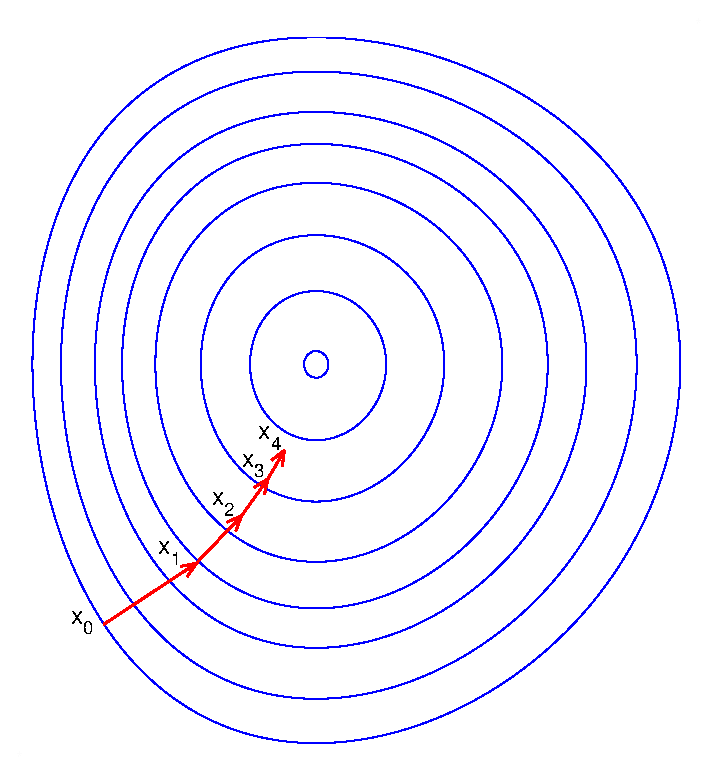
\includegraphics[scale=0.6]{imagens/Gradient_descent.eps}
\caption{Os círculos na imagem representam a função de perda quando há
  apenas 2 parâmetros de peso como exemplo, a função será maior em
  algumas áreas e menor em outras. Tentaremos encontrar os pesos que
  fazem com que a perda seja reduzida. Portanto o método do Gradiente
  irá calcular a derivada da perda em relação aos parâmetros de peso e
  dar um passo na direção oposta ($x_0,x_1,...,x_n$), que significa
  calcular novos pesos para minimizar a perda.}
\label{fig:gradient_descent}
\end{figure}

\section{Aprendizado em profundidade}

O aprendizado em profundidade permite que modelos computacionais
compostos por múltiplas camadas de processamento possam aprender
representações de dados com múltiplos níveis de abstração\cite{LeCun}.
Essa técnica de aprendizado começa a ficar mais famosa depois de 2
adventos específicos da computação: a geração de enormes volumes de
dados e a utilização de GPUs para propósitos gerais (GPGPU).

A solução de \textit{Deep learning} permite que computadores aprendam
a partir de experiências e entendam o mundo em termos de uma
hierarquia de conceitos, com cada conceito definido em termos da sua
relação com conceitos mais simples. Juntando conhecimento de
experiência, essa abordagem evita a necessidade de ter operadores
humanos especificando formalmente todo o conhecimento que o computador
precisa. A hierarquia de conceitos permite que o computador aprenda
conceitos complexos construindo-os à partir de conceitos mais
simples. Desenhando um gráfico que mostra como esses conceitos são
construídos em cima de outros, o gráfico fica profundo, com muitas
camadas. Por esta razão, essa abordagem para IA é chamada de
Aprendizado em profundidade\cite{Goodfellow-et-al-2016-Book}.

\subsection{Otimização com SGD}

O algoritmo SGD (do inglês, \textit{Stochastic Gradient Descent}) é
uma peça chave de \textit{Deep learning}. Praticamente todo o
aprendizado em profundidade é alimentado por esse algoritmo muito
importante. O problema do método do Gradiente visto anteriormente, é
que o mesmo se torna muito difícil de escalar. Para cada vez que é
calculada a perda do modelo, um computador pode levar em torno de 3
vezes esse tempo para calcular o gradiente.

Como foi dito anteriormente, um ponto crucial do aprendizado em
profundidade é a utilização de uma grande quantidade de dados. Visto o
tempo e a ineficiência do método do Gradiente, no algoritmo SGD é
feita uma adaptação para realizar o treinamento sobre um conjunto de
dados maior. Ao invés de calcular a perda, será calculada uma
estimativa dessa perda. Esta estimativa será feita baseada na perda
calculada para uma pequena parte do conjunto de dados do
treinamento. Essa pequena fração terá entre 1 e 1000 exemplos dos
dados e precisa ser escolhida aleatóriamente do conjunto de
treinamento. Utilizando este método, a perda pode aumentar em alguns
momentos, mas isto será compensado pois será possível executar esse
processo muito mais vezes do que com o método do Gradiente
comum. Ao longo do tempo, executar esses procedimentos por milhares ou
milhões de vezes é muito mais eficiente do que utilizar somente o
método do Gradiente.

\subsection{Momentum}

Em cada iteração do processo de treinamento, será tomado um passo bem
pequeno em uma direção aleatória que seria a mais indicada para
diminuir a perda. Mas ao agregar todos esses passos chegamos na função
com perda mínima. É possível tomar vantagem do conhecimento acumulado
de passos anteriores para saber qual direção tomar. Um jeito barato de
fazer isto é manter uma média móvel\footnote{Média móvel é um cálculo
  que analisa pontos de dados criando séries de médias de diferentes
  subconjuntos de um conjunto completo de dados} de todos os
gradientes, e usar essa média móvel ao invés da direção do atual
conjunto de dados. Essa técnica é chamada de \textit{momentum} e
geralmente leva a uma convergência melhor.

\subsection{Declínio da taxa de aprendizado}

Como foi dito anteriormente, em cada etapa do processo de treinamento
é tomado um pequeno passo em direção a minimização da perda. A {\bf
  taxa de aprendizado} é o parâmetro que diz o quão pequeno é esse
passo. Existe uma área inteira de pesquisa sobre essa taxa, e os
melhores resultados indicam que é mais apropriado decair a taxa de
aprendizado em ao longo do treinamento. Neste trabalho iremos aplicar
um declínio exponencial à taxa de aprendizado.\cite{Zeiler}

\subsection{ReLU}

Modelos lineares são simples e estáveis numéricamente mas podem se
tornar ineficientes ao longo do tempo. Portanto para adicionar mais
camadas em nosso modelo, será necessário introduzir alguns cálculos
não lineares entre camadas. Em arquiteturas de profundidade, as
funções de ativação dos neurônios se chamam ReLUs, e são capazes de
introduzir cálculos não lineares aos modelos que possuem mais de uma
camada. Essas são as funções não lineares mais simples que
existem, elas são lineares ($y=x$) se {\bf x} é maior que {\bf 0},
senão ficam iguais a {\bf 0} ($y=0$). Isso simplifica o uso de
\textit{backpropagation} e evita problemas de saturação, fazendo o
aprendizado ficar muito mais rápido.

\begin{figure}[H]
\centering
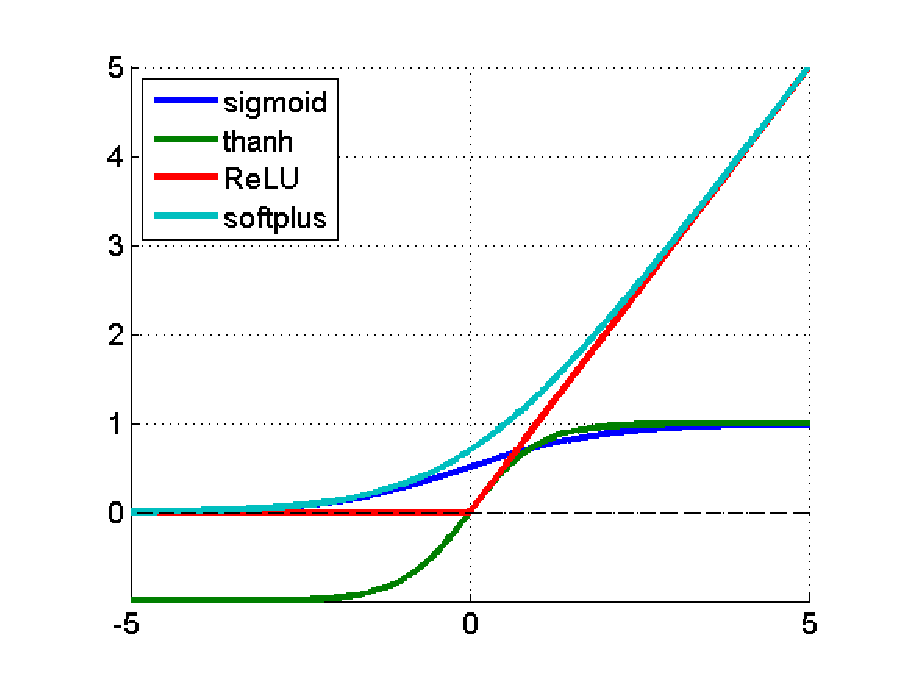
\includegraphics[scale=0.6]{imagens/activation_funcs.eps}
\caption{Comparação de funções de ativação.}
\label{fig:activation_funcs}
\end{figure}

\subsubsection{Camada oculta}

Como as unidades ReLU não precisam de parâmetros e não são observáveis
fora da rede, a introdução dessas unidades entre camadas do modelo é
chamada de camada oculta e pode possuir quantas unidades for
necessário para uma melhor performance.

\subsection{Backpropagation}

\textit{Backpropagation} é um método que faz o cálculo de derivadas de
funções complexas eficientemente, contanto que estas funções sejam
feitas de funções menores que possuem derivadas simples.

\subsubsection{Regra da cadeia}

Um motivo de construir uma rede juntando operações simples é que torna
a matemática muito mais simples. Com a regra da cadeia podemos
concluir que para calcular a derivada de funções compostas, precisamos
apenas calcular o produto das derivadas dos componentes.

Utilizando o método da cadeia, a maioria dos frameworks de aprendizado
de máquina implementa o conceito de \textit{backpropagation}
automaticamente para o usuário. Assim é possível reutilizar dados
pré-calculados e potencializar a eficiência do processo de
treinamento.

\subsection{Regularização}

Regularizar significa aplicar restrições artificiais em sua rede que
fazem com que o número de parâmetros livres reduza e isso não aumente
a dificulade para otimizar.

\subsubsection{Regularização com $L_2$}

A ideia é adicionar um termo a mais à perda, o que dá uma penalidade
em pesos maiores. Essa regularização é atingida adicionando a norma $L_2$
dos pesos a perda, multiplicada por uma constante ($\beta$) de valor
baixo. Esta constante será mais um parâmetro que será necessário
fornecer ao modelo para o treinamento.

\begin{equation}
L' = L + \beta\frac{1}{2} \norm{W}_2^2
\end{equation}

\section{Redes neurais convolucionais de profundidade}

CNNs são a primeira abordagem verdadeiramente bem sucedida em
aprendizado em profundidade onde muitas camadas de uma hierarquia são
treinadas com sucesso de uma maneira robusta. Uma CNN é uma escolha
de topologia ou arquitetura que se aproveita de relações espaciais
para reduzir o número de parâmetros que devem ser aprendidos, e assim
melhora o treinamento diante de uma rede com \textit{feed-forward
  backpropagation}\cite{Arel2010}.

A grande vantagem na abordagem de redes neurais convolucionais de
profundidade (CNN) para reconhecimento é que não é necessário um
extrator de características desenvolvido por um ser humano. Nas
soluções de \cite{Krizhevsky} e \cite{Goodfellow} é possível perceber
que foram usadas diversas camadas para o aprendizado das
características.

Redes neurais convolucionais são muito similares a redes neurais
comuns. De acordo com Karpathy\cite{Karpathy}:
\begin{quote}
  ``Arquiteturas de redes convolucionais assumem explicitamente que as
  entradas são imagens, o que nos permite cifrar algumas propriedades
  dentro da arquitetura. Essas então fazem a função de ativação mais
  eficiente de implementar e reduz drasticamente a quantidade de
  parâmetros na rede.'' (KARPATHY, 2015, tradução nossa).
\end{quote}

Portanto para o caso de reconhecimento de texto em imagens, as redes
neurais convolucionais fazem muito sentido. Ao combinar o aprendizado
em profundidade com redes convolucionais, conseguimos tratar problemas
muito mais complexos de classificação em imagens. Assim problemas mais
simples, como o reconhecimento de textos, podem ser resolvidos cada
vez mais rápido e facilmente.

\subsection{Camada convolucional}

A camada de uma rede neural convolucional é uma rede que compartilha
os seus parâmetros por toda camada. No caso de imagens, cada exemplo
possui uma largura, uma altura e uma profundidade que é representada
pelos canais de cor (Vermelho, Verde e Azul). Uma convolução consiste
em pegar um trecho da imagem de exemplo e aplicar uma pequena rede
neural que teria uma quantidade qualquer de saídas ($K$). Isso é feito
deslizando essa pequena rede neural pela imagem sem alterar os pesos e
montando as saídas verticalmente em uma coluna de profundidade $K$. No
final será montada uma nova imagem de largura, altura e profundidade
diferente. Essa imagem na verdade é um conjunto de {\bf mapas de
  características} da imagem original. Como exemplo, estamos
transformando 3 mapas de carcterísticas (canais de cores) para uma
quantidade $K$ de mapas de características.

Ao invés de apenas Vermelho, Verde e Azul, agora temos uma saída que
possui vários canais de cor. O trecho de imagem é chamado de
\textit{Kernel}, e se for do tamanho da imagem inteira essa seria
igual uma camada comum de uma rede neural. Mas como estamos
trabalhando com este pequeno fragmento, temos bem menos pesos e eles
são todos compartilhados pelo espaço da imagem.

\begin{figure}[H]
\centering
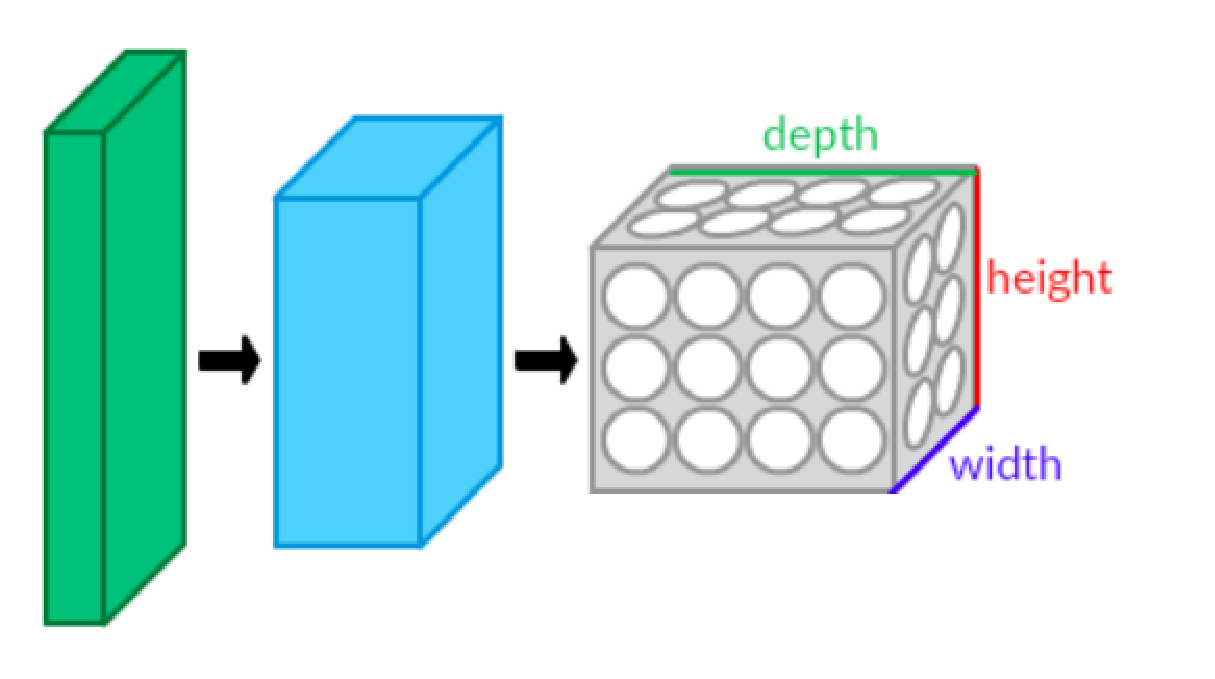
\includegraphics[scale=0.6]{imagens/Conv_layers.eps}
\caption{Para cada convolução, criamos uma nova imagem que possui uma
  nova largura (\textit{width} em inglês), altura (\textit{height} em
  inglês) e profundidade (\textit{depth} em inglês)}
\label{fig:convolution_kernel}
\end{figure}

Uma rede convolucional será basicamente uma rede neural de
profundidade. Ao invés de empilharmos camadas de multiplicação de
matrizes, estamos empilhando convoluções. Portanto no começo teremos
uma imagem grande que possui apenas os valores de pixel como
informação. Assim aplicamos convoluções que irão ``espremer'' as
dimensões espaciais e aumentar a profundidade. No final podemos
conectar nosso classificador e podemos lidar apenas com parâmetros que
mapeiam o conteúdo da imagem.\cite{Dumoulin2016}

\subsubsection{Stride}

Quando estamos realizando uma convolução, deslizamos uma janela com o
tamanho do \textit{Kernel} pela imagem, o \textit{stride} é o
parâmetro que diz quantos pixels de espaçamento teremos entre um
fragmento da imagem e outro. Por exemplo um \textit{stride} de 1
significa que a imagem de saída pode ter a mesma largura e altura que
a imagem de entrada. Um valor de 2 significa que a imagem de saída
pode ter metade do tamanho.

\subsubsection{Padding}

O parâmetro de \textit{padding} é o que se faz nas bordas das imagens
de saída. Uma possibilidade é não deslizar o \textit{Kernel} até as
bordas da imagem, isso é chamado de {\bf \emph{valid padding}}. Outra
possibilidade é deslizar o seu \textit{Kernel} até as bordas da imagem
e completar com 0, essa técnica é chamada de {\bf \emph{same
    padding}}.

\begin{figure}[H]
\centering
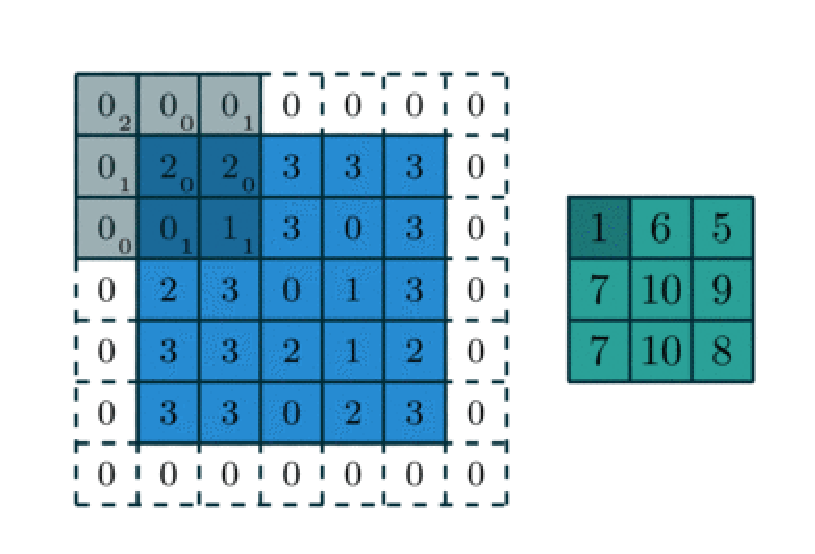
\includegraphics[scale=0.6]{imagens/conv_kernel_pad_stride.eps}
\caption{No exemplo temos uma imagem representada por uma matriz 5x5 e
  está sendo aplicado um \textit{kernel} de tamanho 3x3, com o
  \textit{stride} igual a 2 e um \textit{same padding}, completando as
  bordas com 0. Isso gera uma nova imagem 3x3 por consequência dos
  parâmetros escolhidos.}
\label{fig:convolution_kernel}
\end{figure}

\subsection{Pooling}

Reduzir as dimensões espaciais da nossa rede neural é primordial para
uma arquitetura eficaz do modelo. No entanto utilizar uma convolução
com \textit{stride} igual a 2 para essa tarefa é uma forma agressiva e
arriscada para isso, pois podemos perder bastante informação no
processo. Ao invés disso, iremos realizar convoluções com \textit{stride} igual
a 1, sem perder nenhuma informação da imagem original. Após a camada
convolucional iremos adicionar uma camada de \textit{pooling} que irá
receber todas as convoluções e combiná-las de alguma
forma\cite{Dumoulin2016}.

\subsubsection{Max pooling}

Para cada ponto nos nossos mapas de características essa operação
olha para uma pequena vizinhança ao redor deste ponto. Com esses
valores em mãos é possível calcular o valor máximo dessa vizinhança.

Esta técnica geralmente leva a modelos mais eficazes. Porém a
computação das convoluções com \textit{stride} menor pode se tornar mais
lenta. Além disso, agora será necessário trabalhar com mais parâmetros
para nossa rede neural, o tamanho de região de \textit{pooling} e o parâmetro
de \textit{stride} para o \textit{pooling}.


\chapter{Proposta de experimento}

Para realizar o experimento será necessário treinar um modelo de rede
neural que seja capaz, ou esteja próximo, de decifrar um CAPTCHA. Para
isso serão efetuadas três etapas básicas e comuns quando se trabalha
com redes neurais. Primeiro será coletado o maior número possível de
imagens de CAPTCHA. Em seguida será gerado um dataset com as
características dessas imagens junto com a classe em que pertence. A
partir daí podemos realizar a configuração e treinamento da rede
neural. E por fim será testada a acurácia do modelo mediante imagens
de teste.

\section{Coleta de imagens}

Como o escopo do trabalho não contempla a automatização da recuperação
de informações de websites públicos, foi disponibilizado um
repositório com as imagens necessárias. Esse repositório possui
188.564 imagens e foi disponibilizado pela empresa Neoway. As imagens
se tratam de um CAPTCHA publicado pelo site do SINTEGRA de Santa
catarina
(\url{http://sistemas3.sef.sc.gov.br/sintegra/consulta_empresa_pesquisa.aspx}).

\begin{figure}[H]
\centering

\includegraphics[scale=1]{imagens/exemplo_captcha}
\caption{Um exemplo do CAPTCHA utilizado pelo sistema de consulta do
  SINTEGRA de Santa Catarina.}
\label{fig:gradient_descent}
\end{figure}


\subsection{Fonte pública}

Para demonstrar a ineficiência de certas imagens de CAPTCHA foi
escolhido um software Web. Este software do SINTEGRA, fornece dados
públicos de contribuintes mediante consulta via website. O SINTEGRA é
o Sistema Integrado de Informações sobre Operações Interestaduais com
Mercadorias e Serviçoes. Esta fonte pública possui dados fornecidos
pelos próprios contribuintes na hora do cadastro. Os comerciantes ou
profissionais autônomos fazem seu cadastro para facilitar o comércio
de produtos e prestação de serviços. O cadastro contempla inscrição da
pessoa física ou jurídica, endereço e informações complementares
referentes ao fisco estadual.

\section{Geração do Conjunto de dados}

O conjunto de dados (ou ``dataset'') que alimenta a rede neural é
gerado em tempo de execução do treinamento. Cada imagem é lida de seu
diretório em disco e carregada na memória como uma matriz de valores
de pixel. Ao final deste processo há um vetor em memória com todas
imagens existentes já pré-processadas. Isso é feito para o dataset de
treinamento e de teste. O dataset de treinamento terá a maioria das
imagens, portanto {\bf 180 mil}.

\subsection{Pré-processamento}

A fase de pré-processamento das imagens é mínima e é feita junto com a
geração do conjunto de dados.

\begin{itemize}
\item{\bf Escala de cinza}

Ao gerar um array representativo da imagem, apenas é considerado um
valor de escala de cinza da imagem, assim padronizando os valores de
intensidade de pixels entre 0 e 1.

\item{\bf Redimensionamento}

Ao gerar o array que representa a imagem, é feito um cálculo para
diminuir a imagem com base em uma escala. Essa escala será configurada
à partir de um valor padrão para a largura e altura das imagens.

\end{itemize}

\subsection{Conjunto de dados de teste}

Para o treinamento será necessário um conjunto separado para teste que
não possui nenhuma imagem presente no conjunto de treinamento.
O dataset de testes terá uma amostra bem menor que o conjunto de
treinamento. Portanto terá {\bf 8 mil} imagens.

\section{Treinamento}

Após gerado o conjunto de dados, é possível trabalhar no treinamento
do modelo da rede neural. Para isso será usado o Framework {\bf
  TensorFlow}\cite{TensorFlow} destinado à \textit{Deep Learning} e um
script em Python que fará uso das funções disponibilizadas pela
biblioteca do TensorFlow. Assim realizando o treinamento até atingir
um valor aceitável de acerto no conjunto de teste. O resultado do
treinamento será um arquivo binário representando o modelo que será
utilizado para avaliação posteriormente.

\subsection{Infraestrutura}

Com o intuito de acelerar o processo, foi utilizada uma
máquina com {\bf GPU} para o treinamento. A máquina foi adquirida em
uma \textit{Cloud} privada da AWS. A GPU utilizada se trata de uma
\textit{NVIDIA K80} com 2.496 cores e 12GB de memória de vídeo. Como
processador a máquina possui um \textit{Intel Xeon E5-2686v4
  (Broadwell)} com 4 cores, e ainda possui 61GB de memória RAM
\cite{GPUinstance}.

\subsection{Bibliotecas utilizadas}

Todo o código foi implementado utilizando a linguagem de programação
{\bf \emph{Python}}, e as seguintes bibliotecas foram utilizadas:

\begin{itemize}

\item {\bf TensorFlow}\cite{TensorFlow}: Um Framework implementado em
  \textit{Python} destinado à \textit{Deep Learning}. Proporciona a criação da
  arquitetura e automatização do processo de treinamento de redes
  neurais com \textit{backpropagation}.

\item {\bf NumPy}\cite{NumPy}: Uma biblioteca em \textit{Python}
  criada para computação científica. Possui um objeto de
  \textit{array} com várias dimensões e várias funções sofisticadas
  para cálculos com algebra linear.

\item {\bf OpenCV}\cite{OpenCV}: Uma biblioteca, implementada em
  C/C++, destinada à computação visual. Utilizada para ler imagens em
  disco e realizar o pré-processamento nas mesmas.

\end{itemize}

\section{Avaliação de acurácia}

Para a avaliação, uma nova amostra de imagens será coletada do mesmo
modo que foram coletadas as imagens para treinamento. Essa amostra
terá uma quantidade maior de imagens do que o conjunto de teste.

Com essas amostra de imagens, será feita a execução do teste do modelo
contra cada uma das imagens, assim armazenando uma informação de erro
ou acerto do modelo. Ao final da execução será contabilizado o número
de acertos e comparado com o número total da amostra de imagens para
avaliação. Resultando assim em uma porcentagem que representa a
acurácia do modelo gerado.


\chapter{Desenvolvimento}

Este capítulo descreve o desenvolvimento do projeto proposto. 
Para a construção e treinamento da rede neural foi implementado um
script em \textit{Python} que possui toda a arquitetura da rede
descrita de forma procedural. O framework \textit{TensorFlow} chama a
arquitetura dos modelos de \textit{Graph} (ou grafo, em português) e o
treinamento da rede neural é feito em uma \textit{Session}.

O projeto é composto por 5 tarefas de implementação: 

\begin{itemize}

\item Desenvolvimento do leitor processador do conjunto de dados.

\item Desenvolvimento da função que monta a rede neural.

\item Configuração da rede neural para otimização dos resultados.

\item Desenvolvimento da etapa de treinamento da rede neural.

\item Desenvolvimento da etapa de teste e acurácia do modelo da rede
  neural.

\end{itemize}

No início foi utilizado como base um código já existente destinado ao
reconhecimento de dígitos em imagens. A partir daí foi construído o
reconhecedor textos do trabalho.

\section{Código fonte utilizado como base} \label{codigoBase}

Como base da implementação deste trabalho, foram utilizados exemplos
de código aberto disponíveis no repositório de códigos do
\textit{TensorFlow}\cite{tensorCode}. No repositório há diversos
tutoriais e exemplos que incentivam o auto aprendizado dos
usuários. Um dos exemplos mais conhecido entre a comunidade é o
reconhecedor de dígitos da base dados MNIST\cite{mnist}.

O reconhecedor utilizado como base funciona apenas para dígitos
isolados em imagens separadas. Para o caso do trabalho em questão
foi necessário adaptá-lo para reconhecer conjuntos com 5 dígitos ou
letras em uma mesma imagem sem passar por um processo de segmentação
antes do treinamento.

\section{Leitura e pré-processamento do conjunto de dados}

Para a leitura das imagens e pré-processamento do conjunto de dados, foi
implementada uma classe chamada \textit{OCR\_data}. Esta classe utiliza
a memória RAM para armazenar o conjunto de dados enquanto é processado
pelo treinamento. Para Inicialização da classe, são necessários alguns
parâmetros:

\begin{itemize}

  \item Número de imagens que deve ser lido do disco.
  \item Diretório onde as imagens estão disponíveis.
  \item Número de classes que um caractere pode ter. Para o caso do
    trabalho esse número é igual a 36 pois cada caractere do CAPTCHA
    utilizado como exemplo pode ser somente uma letra minúscula sem
    acentos de ``a'' à ``z'' (26 letras) ou um número de ``0'' à ``9''
    (10 dígitos).
  \item Tamanho da fração dos dado para cada iteração com treinamento.
  \item Tamanho da palavra contida no CAPTCHA. 5 para nosso caso.
  \item Altura da imagem. Número fixo em 60 para as imagens disponíveis.
  \item Largura da imagem. Número fixo em 180 para as imagens
    disponíveis.
  \item Altura definida para redimensionamento da imagem.
  \item Largura definida para redimensionamento da imagem.
  \item A quantidade de canais de cor.

\end{itemize}

\subsection{Leitura das imagens}

As imagens são carregadas utilizando \textit{OpenCV}\cite{OpenCV} com
o método \textit{imread}. Após a leitura precisamos fixar o seu rótulo
para a utilização no treinamento. Como as imagens já estão nomeadas
com o respectivo conteúdo da sua imagem, só o que precisamos fazer é
um vetor utilizável desse texto. 

Primeiro transformamos cada caractere em um número de 0 à 35. Fazemos
isso recuperando o código ASCII de cada caractere e normalizando a
sequência. Portanto, para os dígitos (0 à 9) que possuem códigos indo
de 48 à 57, subtraímos 48. E para as letras (a à z) que possuem
códigos indo de 97 à 122, subtraímos 87 e ficamos com números de 10 à
35. 

Depois de traduzido o caractere para um número, precisamos criar o
vetor do rótulo através do nosso algoritmo de \textit{One-hot
  encoding}. Para isso criamos 5 vetores, um para cada caractere da
imagem, e cada vetor possui 36 posições. Completamos todas as posições
com 0 e em seguida é atribuído o número 1 para a posição referente ao
carctér. A posição do caractere foi determinada pelo passo anterior,
sendo igual o número correspondente ao caractere.

\subsubsection{Fraçao dos dados para treinamento}

Como em cada iteração do treinamento será recuperado apenas uma fração
dos dados, foi criado um método \textit{next\_batch} na classe
\textit{OCR\_data}. Outra motivação para este método é a necessidade de
recuperar uma amostra aleatória dos dados em cada iteração. 

Portanto temos uma variável global na classe \textit{OCR\_data} que
mantém o estado da posição que estamos no conjunto de dados. Após
passar por todo o conjunto de dados, nosso método começa a fazer feita
uma permutação aleatória para garantir que as posições recuperadas do
conjunto de dados sejam completamente escolhidas ao acaso.

\subsection{Pré-processamento das imagens}

Como foi dito anteriormente, a fase de pré-processamento é mínima e
requer apenas alguns parâmetros. Essa etapa é necessária para garantir
uma velocidade maior no treinamento e também garantir uma eficiência
maior como veremos a seguir.

\subsubsection{Quantidade de canais de cor}

No contexto do trabalho, não nos importamos com a cor de um caractere
da imagem. Uma letra ``A'' pode ser vermelha, azul ou verde mas ainda
terá que ser reconhecido como letra ``A''. Com isso em mente podemos
reduzir a quantidade de informações que nosso modelo precisa
aprender. É reduzido também a complexidade dos cálculos feitos pelo
modelo. Quando fazemos a leitura da imagem com a biblioteca OpenCV,
indicamos um parâmetro que diz que a imagem deve ser lida em escala de
cinza (\textit{IMREAD\_GRAYSCALE}). A escala de cinza de uma imagem
representa para cada valor de pixel uma média dos valores de cor RGB
da imagem. Para cada pixel é somado o valor de vermelho com os valores
de verde e azul e dividido por 3. Com isso podemos normalizar nossos
dados de entrada para um valor entre 0 e 1, onde 0 seria um ponto
completamente preto e 1 seria branco.

\subsubsection{Tamanho da imagem}

Outro modo de reduzir informações desnecessárias é redimensionando a
imagem. Com a biblioteca \textit{OpenCV} fazemos isso invocando a
função \textit{resize}. Nessa função passamos como parâmetro a largura
e altura alvos, assim como o algoritmo que deve ser usado para a
interpolação\footnote{Interpolação se trata do algoritmo utilizado
  para redimensionar a imagem. Esse algoritmo irá interpolar cada
  valor de pixel da imagem para obter uma nova imagem
  redimensionada.}. Foi escolhido tamanho de 88 de largura por 24 de
altura pois esses valores correspondem a mais ou menos metade da
imagem. Na seção de arquitetura da rede, também veremos que esses
valores se encaixarão mais naturalmente no nosso modelo. Como
algoritmo de interpolação foi escolhido a reamostragem utilzando a
relação da área de pixel (opção \textit{INTER\_AREA} do
\textit{OpenCV}). Este algoritmo é o indicado pela própria biblioteca
para reduzir imagens. Agora com menos dados a ser processados o
treinamento terá uma velocidade maior.

Ao final da geração de conjunto de dados criamos dois \textit{arrays}
multidimensionais com a biblioteca \textit{NumPy}. Um \textit{array} é das
imagens e terá a forma $quantidade\_de\_imagens\ x\ 88\ x\ 24\ x\ 1$,
sendo a quantidade fornecida como parâmetro, 88 x 24 a largura e
altura da imagem, e 1 é nossa quantidade de canais de cor (ou
profundidade). O outro \textit{array} é para os rótulos e terá a forma
$quantidade\_de\_imagens\ x\ 180$, sendo a quantidade fornecida como
parâmetro e 180 o tamanho do vetor do rótulo pois se trata de 36
classes possíveis multiplicado por 5 caracteres.

\section{Arquitetura da rede neural}

O desenvolvimento da arquitetura da rede neural foi realizado criando
a função \textit{ocr\_net}, que é responsável por especificar o grafo
da rede neural. Essa função irá receber as imagens de entrada, a
quantidade de pesos em cada camada e a quantidade de \textit{biases}
para cada camada.

A arquitetura implementada começa com uma camada de entrada, possui 4
camadas convolucionais, 1 camada completamente conectada e mais uma
camada completamente conectada de saída com 5 saídas, uma para cada
caractere da imagem. Entre uma e outra camada convolucional há uma
camada de ativação (ReLu) e uma camada de \textit{pooling}. Ao final
da última camada convolucional e antes da camada de saída há uma
camada de \textit{dropout}, resultando em um total de 14 camadas sendo
11 visíveis e 3 ocultas.

\begin{figure}[H]
\centering
\includegraphics[scale=0.4]{imagens/training_graph}
\caption{Arquitetura geral do modelo de rede neural treinado.}
\label{fig:training_graph}
\end{figure}

\subsection{Entradas}

Nosso grafo começa com dois parâmetros de entrada, as imagens de
entrada e os rótulos correspondentes. Para esses parâmetros criamos
\textit{placeholders} disponibilizados pelo framework. Esses
\textit{placeholders} inicialmente precisam saber qual tipo dos dados
serão inseridos e o formato final. O tipo dos dados são os valores
normalizados dos pixels das imagens portanto serão pontos
flutuantes. O formato é o que foi definido em nossa classe do conjunto
dos dados ($quantidade\_de\_imagens\ x\ 88\ x\ 24\ x\ 1$ para as
imagens e $quantidade\_de\_imagens\ x\ 180$ para os rótulos).

\subsection{Camadas}

Para melhor visualização e compreensão da arquitetura será descrita
cada camada utilizada por ordem de sequência da entrada até a saída.

\begin{enumerate}

\item Camada de entrada: um \textit{array} multidimensional de formato
  {\bf 88x24x1} que será alimentado com os valores da imagem.

\item Camada convolucional (1): tem como entrada a imagem carregada na
  camada de entrada com {\bf 1} de profundidade. Executa convoluções
  aplicadas à imagem com um \textit{kernel} de formato $5x5$ e {\bf
    64} valores de profundidade. Seu valor de \textit{stride} é igual
  a {\bf 1} e utiliza \textit{same padding}. Por fim é adicionado um
  \textit{bias} de {\bf 64} valores à convolução. O formato do \textit{array}
  multidimensional desta camada é {\bf 88x24x64}.

\item Camada oculta (1): utiliza {\bf ReLU} como função de ativação e
  não recebe nenhum parâmetro. Tem como entrada a camada convolucional
  anterior.

\item Camada de \textit{pooling} (1): executa a operação de
  \textit{max pooling} com um \textit{kernel} de formato $2x2$ e
  \textit{stride} igual a {\bf 2}. Essa operação tem como entrada a
  imagem gerada pelas convoluções após passar pela função de
  ativação. Isso irá reduzir o tamanho desta imagem pela metade. O
  formato do \textit{array} multidimensional desta camada é {\bf 44x12x64}.

\item Camada convolucional (2): tem como entrada a imagem gerada
  nas camadas anteriores com {\bf 64} de profundidade. Executa
  convoluções aplicadas à imagem com um \textit{kernel} de formato
  $5x5$ e {\bf 128} valores de profundidade. Seu valor de
  \textit{stride} é igual a {\bf 1} e utiliza \textit{same
    padding}. Por fim é adicionado um \textit{bias} de {\bf 128}
  valores à convolução. O formato do \textit{array} multidimensional desta
  camada é {\bf 44x12x128}.

\item Camada oculta (2): utiliza {\bf ReLU} como função de ativação e
  não recebe nenhum parâmetro. Tem como entrada a camada convolucional
  anterior.

\item Camada de \textit{pooling} (2): executa a operação de
  \textit{max pooling} com um \textit{kernel} de formato $2x2$ e
  \textit{stride} igual a {\bf 2}. Essa operação tem como entrada a
  imagem gerada pelas convoluções após passar pela função de
  ativação. Isso irá reduzir o tamanho desta imagem pela metade. O
  formato do \textit{array} multidimensional desta camada é {\bf 22x6x128}.

\item Camada convolucional (3): tem como entrada a imagem gerada
  nas camadas anteriores com {\bf 128} de profundidade. Executa
  convoluções aplicadas à imagem com um \textit{kernel} de formato
  $5x5$ e {\bf 256} valores de profundidade. Seu valor de
  \textit{stride} é igual a {\bf 1} e utiliza \textit{same
    padding}. Por fim é adicionado um \textit{bias} de {\bf 256}
  valores à convolução. O formato do \textit{array} multidimensional desta
  camada é {\bf 22x6x256}.

\item Camada oculta (3): utiliza {\bf ReLU} como função de ativação e
  não recebe nenhum parâmetro. Tem como entrada a camada convolucional
  anterior.

\item Camada de \textit{pooling} (2): executa a operação de
  \textit{max pooling} com um \textit{kernel} de formato $2x2$ e
  \textit{stride} igual a {\bf 2}. Essa operação tem como entrada a
  imagem gerada pelas convoluções após passar pela função de
  ativação. Isso irá reduzir o tamanho desta imagem pela metade. O
  formato do \textit{array} multidimensional desta camada é {\bf 11x3x256}.

\item Camada convolucional (4): tem como entrada a imagem gerada
  nas camadas anteriores com {\bf 256} de profundidade. Executa
  convoluções aplicadas à imagem com um \textit{kernel} de formato
  $3x3$ e {\bf 512} valores de profundidade. Seu valor de
  \textit{stride} é igual a {\bf 1} e utiliza \textit{same
    padding}. Por fim é adicionado um \textit{bias} de {\bf 512}
  valores à convolução. O formato do \textit{array} multidimensional desta
  camada é {\bf 11x3x512}.

\item Camada de \textit{dropout}: tem como entrada a camada
  convolucional anterior e possui um formato {\bf 11x3x512}. Recebe o
  valor de {\bf 0.75} como parâmetro de probabilidade de manter cada
  peso da rede neural.

\item Camada completamente conectada: tem como entrada todas as
  ativações das camadas anteriores. Para habilitar nossa camada
  completamente conectada precisamos realizar uma reformatação na
  matriz de entrada. Como a última camada possui um formato de {\bf
    11x3x512}, multiplica-se esses valores para que ao invés de
  ter uma matriz, tenha-se um vetor de tamanho {\bf 16896} como
  entrada. Assim nossa camada completamente conectada terá {\bf 16896}
  ativações de entrada e {\bf 4096} ativações de saída.

\item Camadas completamente conectadas de saída: cada camada terá como
  entrada as {\bf 4096} ativações da camada anterior. E cada saída
  será um vetor de {\bf 36} posições que corresponde às probabilidades
  de classe para cada caractere. No total serão 5 camadas paralelas
  agregadas em uma.

\end{enumerate}

\section{Configuração da rede neural}

Parâmetros fornecidos para a configuração do treinamento da rede
neural são chamados de {\bf hiperparâmetros}. Dependendo da
arquitetura utilizada, uma rede neural pode ter uma quantidade
diferente de hiperparâmetros. A maioria dos hiperparâmetros utilizados
no trabalho foram indicados em artigos citados ao longo da sessão, ou
vieram dos exemplos e tutoriais citados na seção
\ref{codigoBase}. Alguns parâmetros foram modificados ao longo dos
testes.

\subsection{Quantidade de ativações}

Os números de ativações 64, 128, 256, 512 e 4096 nas saídas das
camadas foram utilizados com base em estudos anteriores feitos sobre
redes convolucionais\cite{Krizhevsky}.

\subsection{Tamanho do Kernel}

Baseado nos estudos de \cite{Goodfellow}, foi escolhido um formato
de $5x5$ para o tamanho do \textit{kernel} para a maioria das
camadas. Para a última camada convolucional foi escolhido o tamanho
de $3x3$ pois o \textit{kernel} não pode ter uma dimensão maior que
a imagem de entrada. Como na última camada recebemos uma imagem no
formato $11x3$, não é possivel aplicar convoluções de tamanho $5x5$.

\subsection{Parâmetros do declínio exponencial da taxa de aprendizado}

Ao utilizar uma taxa de aprendizado decadente no otimizador, são
fornecidos alguns parâmetros relativos ao processo de decadência da
taxa. Os valores fornecidos tem como base um dos treinamentos de rede
neural disponível em \cite{tensorCode}.

\begin{itemize}
  
  \item {\bf taxa de aprendizado inicial
      (\emph{initial\_learning\_rate}):} é fornecido um valor de
    {\bf 0,01} para a taxa de aprendizado no início do treinamento.

  \item {\bf passos para decair (\emph{decay\_steps}):} valor que
    indica a cada quantos passos a taxa de aprendizado deve
    diminuir. Esse valor é de {\bf 1.000} passos para o caso do
    trabalho.

  \item {\bf taxa de decadência (\emph{decay\_rate}):} valor referente
    ao quanto a taxa de aprendizado deve decair. Foi escolhido {\bf
      0,9} para o caso do trabalho, portanto a taxa de aprendizado vai
    cair 10\% a cada 1.000 passos do treinamento.

\end{itemize}

\subsection{Momentum}

A estratégia de \textit{momentum} de nosso treinamento precisa de uma
variável que será o fator determinante para o cálculo do gradiente. O
valor dessa variável recomendado pela maioria dos estudos e exemplos é
igual a {\bf 0,9} e é o valor utilizado no treinamento proposto.

\subsection{Regularização com $L_2$}

Como foi dito no capítulo de fundamentação teórica, um parâmetro de
regularização pode ser adicionado a perda do treinamento. Além da
norma $L_2$ calculada baseada nos pesos, esse valor é multiplicado por
uma variável $\beta$ que tem valor igual a {\bf 0,0003} para o
treinamento feito neste trabalho.

\subsection{Probabilidade do Dropout}

Cada valor das ativações terá uma probabilidade de ser mantido ou
não. Como já foi contemplado na explicação do \textit{dropout}, cada
ativação pode ser removida entre uma camada e outra. Para os
treinamentos realizados, foram utilizados dois valores como
tentativa. O primeiro valor foi de {\bf 0,75} e o segundo foi {\bf
  0,5}, isso dá 75\% e 50\% das ativações mantidas respectivamente. O
segundo valor foi empregado na tentativa de minimizar o problema de
\textit{overfitting}.

\subsection{Tamanho da carga em cada passo}

Na otimização com SGD é fornecido um pedaço do conjunto de dados
total em cada passo que calcula-se o método do gradiente. Este pedaço
dos dados será chamado de ``carga'' (ou \textit{batch} em inglês) para
o presente contexto. Baseado em exemplos anteriores, foi escolhido um
valor de {\bf 64} imagens para o tamanho de carga.

\subsection{Número de iterações}

O número de iterações consiste basicamente na quantidade de exemplos
que será calculado o gradiente. Este número leva em consideração o
tamanho da carga e dá o resultado do número de passos que serão
executados no treinamento. Para os treinamentos realizados neste
trabalho foram escolhidos dois valores, um com {\bf 200 mil} iterações
outro com {\bf 500 mil} iterações. Portanto para um treinamento
haverá {\bf 3.125} ($200.000 / 64$) passos e para os outros haverá
{\bf 7.812} ($500.000 / 64$) passos.

\section{Fase de treinamento} \label{treino}

A fase de treinamento é o momento onde se junta todas as peças da
arquitetura e configuração da rede neural. Na implementação foi
criada uma função \textit{train} que é responsável por montar de fato
o grafo para a rede e utilizar o objeto \textit{Session} do
\textit{TensorFlow} para o treinamento.

\subsection{Criação da sessão de treinamento}

O desenvolvimento começa com a abertura da sessão de treinamento. Esta
sessão será destruída ao final das iterações para limpar todas as
variáveis de treinamento carregadas em memória. Após a abertura da
sessão é chamada a função \textit{ocr\_net} para que seja instanciada a
arquitetura da rede neural. Todas as variáveis instanciadas até o
momento de execução da sessão são apenas espaços reservados, assim
como os \textit{placeholders} criados para os dados de entrada do
modelo. Com a arquitetura em mãos será calculada a perda, realizando
uma soma das perdas para cada caractere de saída da rede neural. Em
seguida é instanciado o otimizador (\textit{MomentumOptimizer}) e por
final as predições são agregadas em uma matriz transposta para que
fiquem com o formato $5x36$ (5 caractéres por 36 classes).

\subsection{Inicialização da sessão de treinamento}

Para inicializar a sessão de treinamento é invocado o método
\textit{initialize\_all\_variables} para popular os espaços reservados
das variáveis. Com isso é possível executar a sessão pela primeira vez
invocando \textit{session.run} passando como parâmetro o retorno de
\textit{initialize\_all\_variables}.

\subsection{Execução da sessão de treinamento}

Para manter o controle do treinamento é criada uma variável
\textit{step} que irá manter o estado da quantidade de passos
executados em cada execução da sessão. Para cada passo é invocado o
método \textit{next\_batch} da instância da classe \textit{OCR\_data}
referente ao treinamento. Também será invocado \textit{session.run}
passando como parâmetro o otimizador e carga de dados através de um
dicionário chamado \textit{feed\_dict}. Esse dicionário receberá o
retorno do método \textit{next\_batch} e com isso é possível popular
os \textit{placeholders} da carga de imagens e de seus respectivos
rótulos.

Em cada passo executado é calculada a perda para o treinamento. E a
cada 100 passos é calculada a acurácia para a sessão de treinamento. A
execução do treinamento fica em ciclos até que o número de passos
multiplicado pela quantidade de carga (64) seja igual ao número de
iterações (200 mil ou 500 mil). Ao final de todas as iterações é
instanciado um \textit{Saver}, o qual fará a escrita das variáveis de
nosso modelo em um arquivo. Este arquivo será utilizado para a
avaliação da acurácia em situações reais.

\section{Fase de teste} \label{faseTeste}

A implementação da fase de teste consiste na execução de apenas um
passo da sessão aberta na seção \ref{treino}. Ao final da otimização
do modelo, é carregado o conjunto de imagens para teste, assim como os
respectivos rótulos. A carga é feita utilizando o método
\textit{next\_batch} da instância da classe \textit{OCR\_data}
referente ao teste. Com isso é possível popular o dicionário
\textit{feed\_dict} da sessão de teste e executar \textit{session.run}
com este parâmetro. Ao final teremos o valor da acurácia e da perda
para o conjunto de dados do teste.

\subsection{Acurácia}

O cálculo da acurácia para o modelo é o mesmo tanto para a fase de
treinamento quanto para fase de teste. A função de acurácia recebe
como parâmetro a matriz de predições gerada pelo modelo e a matriz de
rótulos fornecida pela carga dos dados. O cálculo é feito armazenando o
maior valor de cada \textit{array} da matriz de predições e comparando
as posições desses valores com as posiçõs da matriz de rótulos. A
acurácia sobe para cada letra certa em uma imagem de CAPTCHA, sem
levar em consideração se todas as letras estão certas ou não.


\chapter{ Testes }

Neste capítulo são apresentados os testes realizados no sistema
proposto com a arquitetura de rede neural definida no capítulo
anterior.



\chapter{ Conclusões }

Para desenvolver o projeto foi escolhido o software que até a presente
data é o mais recomendado para tarefas de aprendizado de máquina. Um
reconhecedor de texto em imagens de CAPTCHA foi desenvolvido ao longo
do trabalho. Este reconhecedor conta com um alto nível de robustez
diante dos testes realizados.

Os testes realizados em todos os casos mostraram ser possível atingir um
resultado razoável na tarefa de reconhecimento de textos em imagens,
isso com poucos ajustes à configuração de treinamento de redes
neurais. Atualmente a quantidade de exemplos e tutoriais disponíveis
para tarefas de aprendizado de máquina é imenso. Fica claro que é
possível implementar classificadores mesmo com poucos recursos.

\section{Vulnerabilidade de fontes públicas}

Diante do objetivo alcançado pelo trabalho, fica aparente que fontes
públicas de dados podem estar vulneráveis. Consultas automatizadas
realizadas por \textit{Web crawlers} podem não afetar diretamente a
segurança das informações, isso porque as informações já estão sendo
disponibilizadas publicamente. Entretanto a disponibilidade de tais
fontes pode ser afetada quando o ambiente de um \textit{website} não
está preparado para um volume muito grande de consultas.

\subsection{Eficácia de CAPTCHAs}

Enquanto é possível discutir a eficácia dessas imagens de CAPTCHA e
como gerar imagens mais difíceis de se reconhecer, também cabe uma
discussão sobre a necessidade de imagens na tentativa de bloquear
consultas automatizadas. Imagens usadas como CAPTCHA geralmente são
frustrantes para usuários humanos de sistemas de consulta. Ao tentar
dificultar o reconhecimento de imagens por máquinas, também se
dificulta o acesso de um usuário comum às informações. Portanto é
possível abrir espaço para estudos que buscam outras formas de
bloqueio de \textit{Web crawlers}.

Outra alternativa, inclusive mais interessante, seria
disponibilizar outros tipos de consulta específicos para sistemas de
terceiros que desejam utilizar dados públicos. Assim um
\textit{website} de fonte pública de dados poderia continuar a servir
usuários humanos com robustez e ao mesmo tempo servir usuários
sistêmicos com um formato mais adequado.

\section{Trabalhos futuros}

Como possíveis trabalhos futuros, cita-se: 

\begin{itemize}

        \item Fazer um melhor uso das informações geradas pelo
          processo de treinamento para gerar heurísticas mais
          inteligentes. Um exemplo seria utilizar outros tipos de
          otimizadores para a função da perda.

        \item Estender o sistema para realizar o reconhecimento de
          outros tipos de CAPTCHAs.

        \item Estender o sistema para realizar o reconhecimento de
          tipos de CAPTCHAs que possuem um tamanho de texto variável.

        \item Realizar um estudo sobre \textit{Web crawlers} em fontes
          públicas que utilizam CAPTCHA, executando o sistema proposto
          neste trabalho.

        \item Implementar um sistema de reconhecimento de CAPTCHAs
          mais avançados que solicitam a classificação de uma cena
          completa ou identificação de objetos em imagens.

        \item Estudar um artifício mais efetivo para o bloqueio de
          consultas automatizadas em \textit{websites}.

\end{itemize}

Considera-se de extrema importância a implementação de projetos desse
tipo pois o mesmo auxilia na compreensão e aplicação de Inteligencia 
Artificial em casos específicos.

\bibliography{ref}

\end{document}
